\chapter{Solids, Liquids, Gases}\label{ch:g3:solids-liquids-gases}

A stone, a glass of milk, the \omterm{def:g2:air-around-us:air}{air} in a balloon: three kinds of stuff
that behave in three utterly different ways. Last year, water showed
us its three states; this year we discover that \emph{everything}
is in one of these three states --- and each state has strict
rules.

\section{Three families of stuff}

All the stuff in the world can be sorted into three families, called
the three \emph{states}: \omterm{def:g3:solids-liquids-gases:solid}{solid} like the stone, \omterm{def:g3:solids-liquids-gases:liquid}{liquid} like the milk,
\omterm{def:g3:solids-liquids-gases:gas}{gas} like the \omterm{def:g2:air-around-us:air}{air}. Ice, water and steam were our first example: one
stuff visiting all three families. Now let us learn each family's
rules.

\section{Solids keep their shape}

\begin{definition}[Solid]\label{def:g3:solids-liquids-gases:solid}
A \emph{solid}\index{solid} is stuff that keeps its own shape. A key
keeps its zigzag in your pocket, in a drawer, or underwater. You can
hold a solid between two fingers, and moving it does not change what
it looks like. Some solids are hard (stone), some soft (bread), some
bendy (a rubber band) --- but left alone, each keeps its shape.
\end{definition}

\begin{example}[A solid made of grains]\label{ex:g3:solids-liquids-gases:sand}
Sand seems to break the rule: poured from a bucket, it takes the
shape of its pile, almost like a \omterm{def:g3:solids-liquids-gases:liquid}{liquid}. But look closely: sand is a
crowd of tiny \omterm{def:g3:solids-liquids-gases:solid}{solid} grains, and \emph{each grain} keeps its shape
perfectly. Flour, sugar and rice play the same trick --- crowds of
little \omterm{def:g3:solids-liquids-gases:solid}{solids} that flow together while each member stays \omterm{def:g3:solids-liquids-gases:solid}{solid}.
\end{example}

\section{Liquids flow --- but keep their amount}

\begin{definition}[Liquid]\label{def:g3:solids-liquids-gases:liquid}
A \emph{liquid}\index{liquid} is stuff that flows: it has no shape
of its own and takes the shape of whatever container holds it. But a
liquid keeps its \emph{amount}: pour a full glass of milk into a
bowl and it is still the same amount of milk --- not a drop more or
less, only a new shape.
\end{definition}

\begin{omfigure}
\begin{tikzpicture}[scale=0.85]
  \draw[thick] (0,1.7) -- (0.25,0.1) -- (1.75,0.1) -- (2.0,1.7);
  \fill[omDef, opacity=0.3] (0.14,0.8) -- (1.86,0.8) -- (1.79,0.1)
    -- (0.21,0.1) -- cycle;
  \node[below, font=\small] at (1.0,-0.2) {glass};
  \draw[thick] (4.0,1.1) .. controls (4.1,0.15) .. (5.1,0.1)
    .. controls (6.1,0.15) .. (6.2,1.1);
  \fill[omDef, opacity=0.3] (4.05,0.55) .. controls (4.15,0.18)
    .. (5.1,0.14) .. controls (6.05,0.18) .. (6.15,0.55) -- cycle;
  \node[below, font=\small] at (5.1,-0.2) {bowl};
  \draw[thick] (8.2,1.7) -- (8.2,0.1) -- (11.0,0.1) -- (11.0,1.7);
  \fill[omDef, opacity=0.3] (8.2,0.45) rectangle (11.0,0.1);
  \node[below, font=\small] at (9.6,-0.2) {dish};
  \node[above, font=\small] at (5.5,1.9)
    {the same milk: new shape each time, same amount always};
\end{tikzpicture}

{\small One glassful of milk poured from container to container: the
shape obeys the container, the amount obeys nobody.}
\end{omfigure}

\begin{proposition}[A resting liquid lies level]\label{prop:g3:solids-liquids-gases:level}
The surface of a \omterm{def:g3:solids-liquids-gases:liquid}{liquid} at rest is always flat and level ---
parallel to the floor. Tilt the bottle: the water inside does not
tilt with it; its surface stays level while the bottle leans.
\end{proposition}

\begin{omfigure}
\begin{tikzpicture}[scale=0.85]
  \draw[thick] (0.3,-0.9) rectangle (2.1,1.7);
  \fill[omDef, opacity=0.3] (0.3,-0.9) rectangle (2.1,0.5);
  \draw[omDef, very thick] (0.3,0.5) -- (2.1,0.5);
  \node[below, font=\small] at (1.2,-1.25) {upright};
  \begin{scope}
    \clip[rotate around={-28:(6.2,0.6)}] (5.3,-0.7) rectangle (7.1,1.9);
    \fill[omDef, opacity=0.3] (4.6,-1.1) rectangle (7.8,0.5);
    \draw[omDef, very thick] (4.6,0.5) -- (7.8,0.5);
  \end{scope}
  \begin{scope}[shift={(6.2,0.6)}, rotate=-28]
    \draw[thick] (-0.9,-1.3) rectangle (0.9,1.3);
  \end{scope}
  \node[below, font=\small] at (6.2,-1.25) {tilted: the water stays level};
\end{tikzpicture}

{\small Tilt the bottle as you like: the water's surface refuses to
tilt. A resting \omterm{def:g3:solids-liquids-gases:liquid}{liquid} always lies level.}
\end{omfigure}

\begin{example}[The level at work]\label{ex:g3:solids-liquids-gases:level}
Builders use this law every day: their \emph{spirit level} is a
little window of \omterm{def:g3:solids-liquids-gases:liquid}{liquid} with one bubble; when the bubble sits
between its marks, the shelf is as level as the \omterm{def:g3:solids-liquids-gases:liquid}{liquid} inside. And
at breakfast, watch the juice in a tilted carton: however you tip
it, the surface inside stays flat and level --- until it finds the
spout.
\end{example}

\section{Gases fill everything}

\begin{definition}[Gas]\label{def:g3:solids-liquids-gases:gas}
A \emph{gas}\index{gas} is stuff that spreads out to fill \emph{all}
the room it is given. \omterm{def:g2:air-around-us:air}{Air} is a gas: put it in a bottle, it fills the
bottle to every corner; open the bottle in a bigger room, and it
spreads through that too. A gas has neither its own shape nor its
own resting place --- offer it more room, and it takes everything.
\end{definition}

\begin{example}[The traveling perfume]\label{ex:g3:solids-liquids-gases:perfume}
Someone opens a perfume bottle at one end of the room. A moment
later, noses at the \emph{other} end notice it. The perfume \omterm{def:g3:solids-liquids-gases:gas}{gas} did
not stay politely near its bottle: released, it spread through all
the \omterm{def:g2:air-around-us:air}{air} of the room, corner to corner --- exactly what the \omterm{def:g3:solids-liquids-gases:gas}{gas}
family always does.
\end{example}

\begin{omfigure}
\begin{tikzpicture}[scale=0.85]
  \draw[thick] (0,0) rectangle (11,3.0);
  \draw[thick, fill=omMeth, fill opacity=0.4]
    (0.8,0) rectangle (1.4,0.9);
  \node[below, font=\small] at (1.1,-0.25) {perfume bottle, just opened};
  \foreach \x/\y in {1.6/1.2, 2.1/0.6, 2.5/1.7, 3.2/1.0, 3.9/2.2,
      4.6/0.5, 5.3/1.5, 6.1/2.5, 6.9/0.9, 7.7/1.9, 8.5/0.4,
      9.2/2.3, 9.9/1.2, 10.4/2.7, 5.8/0.3, 8.9/1.4} {
    \fill[omThm, opacity=0.7] (\x,\y) circle (2.2pt);
  }
  \node[above, font=\small] at (8.3,3.1)
    {a little later: perfume everywhere};
\end{tikzpicture}

{\small A \omterm{def:g3:solids-liquids-gases:gas}{gas} on the loose: released in one corner, it spreads until
it fills the whole room.}
\end{omfigure}

\begin{omfigure}
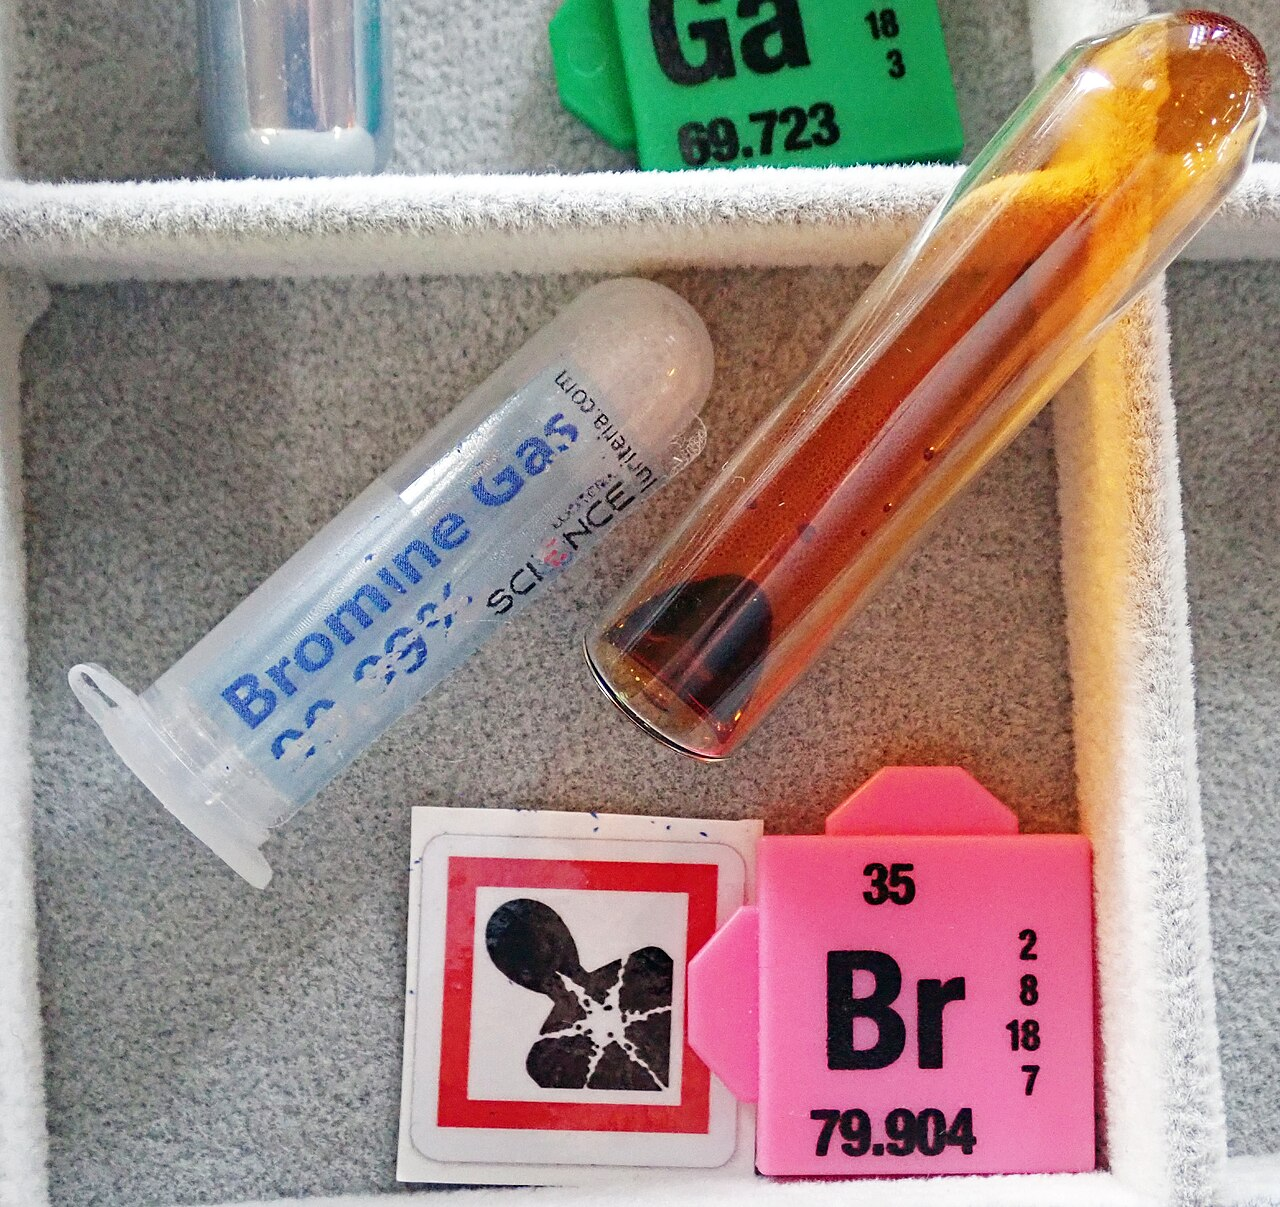
\includegraphics[width=0.4\linewidth, trim={585bp 418bp 15bp 130bp}, clip]
  {images/book1/bromine-gas.jpg}

{\small Most gases are invisible --- but not all. This sealed glass
tube holds bromine, a \omterm{def:g3:solids-liquids-gases:gas}{gas} with a real brown-orange color: you can
\emph{see} it filling every corner of its container, right up to
the glass. \emph{Photo: James St.~John, CC BY 2.0 (cropped).}}
\end{omfigure}

\begin{remark}[Sorting the tricky ones]\label{rem:g3:solids-liquids-gases:tricky}
Some stuff needs a careful eye. Honey flows --- slowly, but it
flows, takes its container's shape and keeps its amount: a \omterm{def:g3:solids-liquids-gases:liquid}{liquid},
just a lazy one. Toothpaste and ketchup flow when squeezed: thick
\omterm{def:g3:solids-liquids-gases:liquid}{liquids}. A sponge is a \omterm{def:g3:solids-liquids-gases:solid}{solid} full of air-filled holes. And smoke?
Tiny \omterm{def:g3:solids-liquids-gases:solid}{solid} specks riding on hot \omterm{def:g3:solids-liquids-gases:gas}{gas}. When in doubt, ask the family
questions: does it keep its shape? does it flow? does it fill all
the room it gets?
\end{remark}

\section{Exercises}

\begin{exercise}[$\star$]\label{exo:g3:solids-liquids-gases:1}
Sort into the three families: a coin; \ orange juice; \ the \omterm{def:g2:air-around-us:air}{air} in a
tire; \ a wooden bead; \ oil; \ the \omterm{def:g3:solids-liquids-gases:gas}{steam-gas} above the clear gap of
a boiling pot.
\end{exercise}

\begin{exercise}[$\star$]\label{exo:g3:solids-liquids-gases:2}
What does a \omterm{def:g3:solids-liquids-gases:solid}{solid} keep that a \omterm{def:g3:solids-liquids-gases:liquid}{liquid} does not? What does a \omterm{def:g3:solids-liquids-gases:liquid}{liquid}
keep when poured from glass to bowl?
\end{exercise}

\begin{exercise}[$\star$]\label{exo:g3:solids-liquids-gases:3}
A full bottle of lemonade is poured into a wide salad bowl. Is there
now more lemonade, less, or the same amount? What changed?
\end{exercise}

\begin{exercise}[$\star$]\label{exo:g3:solids-liquids-gases:4}
Draw a fish tank half full of water: first standing flat, then
tilted up on one edge. Draw the water surface in both --- which way
does it lie?
\end{exercise}

\begin{exercise}[$\star$]\label{exo:g3:solids-liquids-gases:5}
How does a builder's spirit level tell that a shelf is level? Which
law of this chapter is it using?
\end{exercise}

\begin{exercise}[$\star$]\label{exo:g3:solids-liquids-gases:6}
Why does the smell of pancakes reach your bedroom upstairs? Which
family is at work, and what is its rule?
\end{exercise}

\begin{exercise}[$\star$]\label{exo:g3:solids-liquids-gases:7}
Sand pours like a \omterm{def:g3:solids-liquids-gases:liquid}{liquid}, yet we call it \omterm{def:g3:solids-liquids-gases:solid}{solid}. Explain, using
\cref{ex:g3:solids-liquids-gases:sand}.
\end{exercise}

\begin{exercise}[$\star$]\label{exo:g3:solids-liquids-gases:8}
Honey takes a whole minute to flow off the spoon. \omterm{def:g3:solids-liquids-gases:solid}{Solid} or \omterm{def:g3:solids-liquids-gases:liquid}{liquid}?
Ask the family questions of
\cref{rem:g3:solids-liquids-gases:tricky} and answer.
\end{exercise}

\begin{exercise}[$\star$]\label{exo:g3:solids-liquids-gases:9}
Which family: keeps its own shape? \ takes its container's shape but
keeps its amount? \ takes all the room it can get? Give one member
of each family found in your kitchen.
\end{exercise}

\begin{exercise}[$\star\star$]\label{exo:g3:solids-liquids-gases:10}
An ice cube (\omterm{def:g3:solids-liquids-gases:solid}{solid}) \omterm{def:g2:ice-water-steam:meltfreeze}{melts} into water (\omterm{def:g3:solids-liquids-gases:liquid}{liquid}), which the summer sun
dries into invisible flying water (\omterm{def:g3:solids-liquids-gases:gas}{gas}). Which family rule breaks at
each step: what does the stuff stop keeping when ice \omterm{def:g2:ice-water-steam:meltfreeze}{melts}? when
water \omterm{def:g2:ice-water-steam:evapcond}{evaporates}?
\end{exercise}

\begin{exercise}[$\star\star$]\label{exo:g3:solids-liquids-gases:11}
A balloon is blown up and knotted. Mira says the \omterm{def:g2:air-around-us:air}{air} inside is
``balloon-shaped, so a \omterm{def:g3:solids-liquids-gases:gas}{gas} does have a shape''. Explain what is
really giving the shape, and what the \omterm{def:g2:air-around-us:air}{air} would do the instant the
balloon popped.
\end{exercise}
